% =============================================================
%  TubeMethodPaper_body.tex
%  Copernicus (Geochronology) manuscript body, ported from thesis
%  Chapter 1 on 2026-10-30 by Paper/build_paper_from_chapter1.py.
%  Every wording change relative to the thesis is listed in
%  Paper/PORT_CHANGELOG.md. This file is now the source of truth for
%  the paper; edit it directly.
% =============================================================

\providecommand{\tophline}{\toprule}
\providecommand{\middlehline}{\midrule}
\providecommand{\bottomhline}{\bottomrule}

\section{Introduction}

Noble gas geochronology and thermochronometry (\textsuperscript{40}Ar/\textsuperscript{39}Ar and U-Th/He) on hydrous and sulfur-bearing mineral phases such as hornblende, clay minerals, biotite, goethite, and pyrite have already been leveraged as a powerful tool for understanding regional thermal histories as well as the timing of iron or rare metal mineralization \citep{mcinnes2005,heim2006,vasconcelos2013,nomade2004,yakubovich2020,yakubovich2021}. The interpretation of these data, however, is often complicated by the fact that helium (or argon) within hydrous or sulfur-bearing phases often degasses differently in the laboratory and in nature \citep{hanson1975,lee1993,lo2000,farley2024}.

Experiments aiming to characterize the migration mechanisms and rates of noble gases through hydrous phases yield different results when conducted under hydrothermal conditions as opposed to traditional experimental methods in vacuo. Hydrothermal step heat experiments for argon in biotite and hornblende showed higher retentivity and comparatively favored diffusive loss mechanisms relative to experiments conducted in vacuo, and these results are more likely to accurately reflect loss mechanisms in nature \citep{harrison1982,harrison1985}; however, such experiments are labor-intensive and comparatively inflexible relative to modern helium step heat methods \citep{farley1999}.

Recently, some workers have taken advantage of the high helium permeability and selectivity of pure silica glass when designing novel experimental methods for U-Th/He geochronology \citep{yakubovich2020,yakubovich2021}, but these ideas have only been applied in a limited way to characterize helium migration in sulfur-bearing or hydrous phases (e.g., monotonic ramped heating experiments: \citealp{yakubovich2019}). This work aims to apply decades of research on helium permeability, solubility, and diffusion in fused silica glass \citep[e.g.,][]{jones1953,norton1953,rogers1954,altemose1961,swets1961,doremus1966,masaryk1968,shelby1971,shelby1972,shelby1976,shackelford1972} to adapt existing agile step-heat methods \citep{farley1999} to investigate helium loss rates and mechanisms in sulfur-bearing and hydrous mineral phases. 

Encapsulating minerals in silica glass ampoules allows experimentalists to maintain hydrothermal or sulfur-saturated conditions within the ampoule without otherwise altering the experimental design. Depending on the thermodynamics of the phase of interest, this method may stabilize the phase at elevated experimental temperatures, allowing for detailed characterization of helium migration in sulfide and hydrous minerals that hitherto has remained poorly understood.

\section{Method}\label{sec:method}

\subsection{Ampoule Preparation}\label{sec:ampoule-prep}

\begin{figure}[t]
\centering
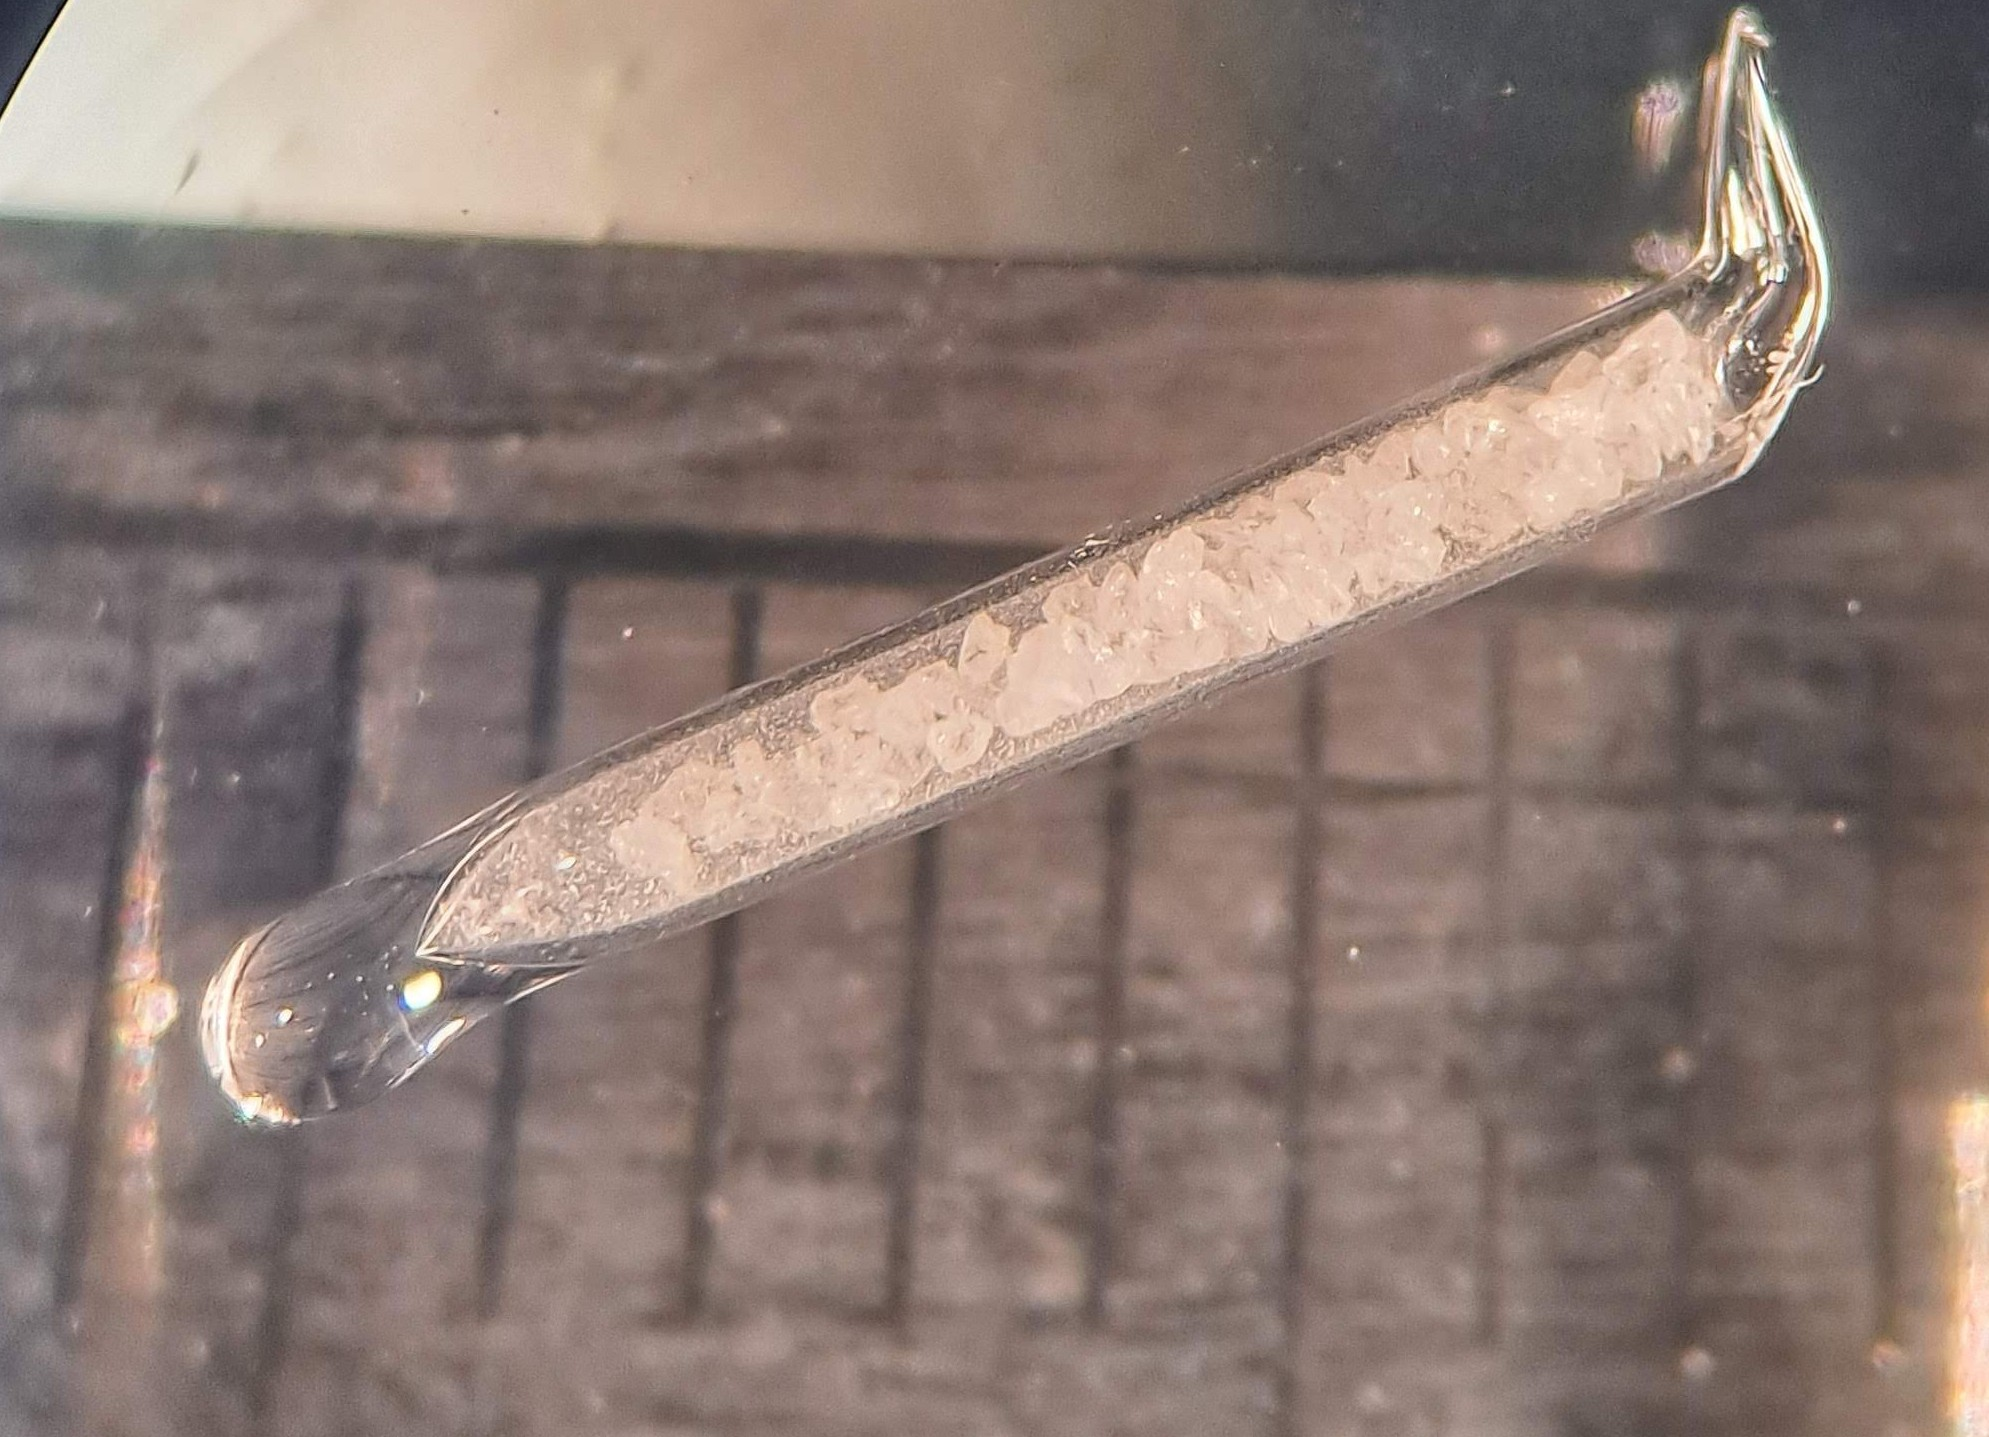
\includegraphics[width=8.3cm]{Apatite_tube.jpg}
\caption{A typical silica glass ampoule used for helium step heat experiments. The ampoule shown here contains Durango Apatite crushate sieved to 300 µm (radii $\approx$ 150 µm). The ampoule is roughly one cm long and one mm wide. The bars visible in the background are each separated by 1 mm.}
\label{fig:ampoule-photo}
\end{figure}

To prepare the silica glass ampoules, \textasciitilde10 cm long segments of pure silica glass tubes with an outer diameter of 4 mm and an inner diameter of 3 mm were submerged and sonicated within acetone, ethanol, then MilliQ water baths in sequence, and then were dried overnight in a 100°C oven. The glass tubes were hand-pulled into thin pipettes with a jewelry welding torch and their thin ends were fused closed (Fig.~\ref{fig:ampoule-photo}).

After the glass had cooled, degassed lab-grade sulfur, distilled water, or Durango apatite were added to some of the tubes. Two tubes were left empty. To seal, the top of each pipette was interfaced with a vacuum line and was pumped to a pressure of \textless0.1 torr. The encapsulated water tube was flash-frozen in liquid nitrogen and then pumped and sealed in a saltwater ice bath to selectively pump away atmospheric gases and not water. Sublimation of sulfur and water ice during pumping was minor. The primary motivation for pumping the tube to rough vacuum was to aid the sealing process. After rough vacuum was achieved, a fine-tipped welding torch was used to seal the top of each ampoule. To determine the geometric factors for permeation of the ampoules, the inner and outer diameters of each ampoule were determined using the measurement function of the Amscope stereo microscope software, which was calibrated and tested during early development of this method.

We found that the fused silica ampoules were capable of maintaining surprisingly high internal pressures, but ampoules filled with water would often explode at temperatures above 315°C. It is recommended that experimentalists limit the temperature of water-filled ampoules to below 300°C. We have not observed any explosions of sulfur-filled ampoules at any temperature. 

\subsection{Permeation Lag}\label{theoretical-framework-of-permeation-lag}

\begin{figure}[t]
\centering
\includegraphics[width=11.8cm]{Schematic_Sequence5.pdf}
\caption{The permeation step method. Each row is one step of an experiment, in time order; the ampoule interior is tinted by step temperature. During experimental steps the sample releases helium (\(\omega\)) into the ampoule, and during every step helium permeates out of the ampoule and is measured (\(m\)). \(n_i\) is the helium in the ampoule at the end of step \(i\). Each permeation step, during which the sample releases no helium, gives the ampoule's helium content at both of its ends (Eq.~\eqref{eq:permsol}), and these bracketing values return \(\omega\) for each experimental step (Eq.~\eqref{eq:permlag}).}
\label{fig:schematic-permstep}
\end{figure}

The process of helium permeation through thin walls of an ampoule is rapid but not instantaneous on 
experimental timescales. Helium evolved from encapsulated minerals is only available for measurement 
following permeation through the glass ampoule (Fig.~\ref{fig:schematic-permstep}), producing a 
predictable ``permeation lag'' effect in helium measurements that commonly manifests with 
undermeasurement of helium during prograde heating sequences and corresponding overmeasurement of 
helium produced during retrograde sequences (supplementary Fig.~\ref{fig:durango-stepwise-yields}). 
This is not merely a theoretical concern: Fig.~\ref{fig:durango-arrhenius-lag-corrected} shows the same 
artifact in real, uncorrected step heat data for the encapsulated Durango apatite experiment described 
in \S\ref{experimental-methods}; the correction developed below is applied to this dataset in full 
in \S\ref{results} (Fig.~\ref{fig:durango-arrhenius-lag-corrected}).

This effect can be modeled (and corrected for) for a system obeying the simple equation:

\begin{equation}
\label{eq:permlag}
n_{t} = n_{0} + \omega - m
\end{equation}

Where \(n_{t}\) is the amount of helium within the ampoule after time \emph{t}, \(n_{0}\) is the initial amount of helium within the ampoule (which is inherited from previous heating steps), \(\omega\) is the amount of helium evolved by the encapsulated sample during time \emph{t,} and \(m\) is the amount of measurable helium that has permeated out of the ampoule into the high-vacuum chamber during time \emph{t.}

Heating steps are consecutive, so the helium inventory quantified between two steps applies to both the previous and the subsequent step. Where steps are numbered, we therefore write \(n_i\) for the helium in the ampoule at the end of step \(i\), so that step \(i\) begins with \(n_{i-1}\) and Eq.~\eqref{eq:permlag} becomes \(\omega_i = m_i + n_i - n_{i-1}\) (Fig.~\ref{fig:schematic-permstep}).

Recovering \(\omega\) for a step therefore requires knowledge of the ampoule's helium content immediately before and immediately after it. Sections~\ref{permeation-step-method} and~\ref{bounding-method} give the two routes used in this work to obtain those quantities.

\begin{figure}[t]
\centering
\includegraphics[width=8.3cm]{encapsulated_DApErr.pdf}
\caption{An Arrhenius plot of a helium step heat experiment of silica-glass encapsulated Durango Apatite with 2$\sigma$ error bars. Without permeation lag corrections, the apparent diffusivities display highly irregular behavior that would be unrecognizable to this well-behaved sample. With permeation lag corrections, the sample agrees well with the reported diffusive parameters of \citet{farley2000} for the appropriate sieve size ($r$ = 150\textmu m). As the experiment proceeds beyond temperatures of 300\textdegree C, the activation energy of diffusion decreases to reveal a slight downward curl, a phenomenon well-documented for Durango apatite likely due to annealing of crystal defects and radiation damage \citep{wolf1996,farley2000}. Apparent diffusivities are calculated with the equations of \citet{fechtigkalbitzer1966} with and without permeation lag corrections. Four measurements of the permeation lag corrected apparent diffusivities are within error of 0 at the 2$\sigma$ level and thus are excluded from the plot.}
\label{fig:durango-arrhenius-lag-corrected}
\end{figure}

Helium permeation through fused silica in diffusive steady state is a first order process that can be described with the simple differential equation:

\begin{equation}
\label{eq:permode}
\frac{dn}{dt} = - \lambda n
\end{equation}

Where \emph{n} is the number of helium atoms, \emph{t} is the time, and \(\lambda\) is the ampoule's permeation rate constant, which depends on the helium permeability of the glass and the geometry of the ampoule (\(\lambda = KGRT\); Supplement, Sect.~\ref{sec:s-lambda-K}). It is easily integrated by separation of variables to yield \(n_{t} = n_{0}e^{- \lambda t}\) (see supplement, \S\ref{a-ficks-law-formulation}, for details). Relating that result to the measured quantity through Eq.~\eqref{eq:permlag} in the absence of any release from the sample \(\left( m(\omega = 0) = n_{0} - n_{t} \right)\) gives an expression most intuitively stated in terms of the fraction of the ampoule's initial helium reservoir that permeates during time \emph{t}:

\begin{equation}
\label{eq:permsol}
^{He}F = \frac{m}{n_{0}} = 1 - e^{- \lambda t}
\end{equation}

Where \(^{He}F\) is the fractional permeation yield: the fraction of the ampoule's initial helium reservoir (\(n_{0}\)) that permeates as \(m\) (Eq.~\eqref{eq:permlag}) during a time \emph{t} of steady state permeation, and \(\lambda\) is the ampoule's permeation rate constant. \(\lambda\) is the quantity that can be measured directly during an experiment (\S\ref{in-situ-rate-constant}).

Equation~\eqref{eq:permsol} is only strictly valid with two assumptions:

\begin{enumerate}
\def\labelenumi{\arabic{enumi}.}
\item
  The helium partial pressure in the ``measurable'' reservoir outside of the ampoule is negligible compared to the partial pressure within the ampoule. Because the ratio of typical ampoule to diffusion cell volumes is \textasciitilde1/10,000 \citep{farley1999}, this assumption is essentially always reasonable.
\item
  The helium concentration profile within the ampoule's glass walls is in diffusive steady state between the inner and outer walls. The real steady state helium concentration profile is well-approximated by the ideal steady state profile for ampoules with a glass/gas volume ratio less than 2 (Figs.~\ref{fig:steady-state-profile-deviation},~\ref{fig:numerical-error-volume-ratio-control}). For these ampoules, \eqref{eq:permsol} is accurate to within 1\% after the establishment of a diffusive steady state. Additionally, the diffusive steady state assumption is ephemerally violated when the temperature is changed due to the temperature dependence of the glass/gas partitioning of helium. The ampoule should therefore be held at the permeation temperature for at least one diffusive timescale \(\tau = L^{2}/D\) after every temperature change before measuring, where \emph{L} is the wall thickness and \emph{D} the diffusivity of helium in silica glass \citep{swets1961}. In this work, low-temperature heating steps are repeated to allow for the new diffusive steady state concentration profile to become established. The ampoules of this work reach diffusive equilibrium in 30--70 minutes at 80°C (Fig.~\ref{fig:diffusive-profile-reequilibration-time}; supplementary Figs.~\ref{fig:fdm-profile-evolution-300-to-100c} and~\ref{fig:fdm-profile-evolution-zero-initial-condition}). Comparisons between the abundance of helium within glass as a function of temperature limit the error introduced by thermal perturbation to less than 5\% (supplementary Fig.~\ref{fig:thermal-perturbation-error}).
\end{enumerate}

From Eq.~\eqref{eq:permlag}, it is immediately clear that when the evolved helium \(\omega\) is large with respect to the amount of helium within the ampoule, \(n_{t}\) or \(n_{0}\), then \(\omega \approx m\) and permeation lag can be neglected. Unfortunately, this is not the case for most phases commonly subjected to helium step heat experiments with routine heating schedules (e.g. hour-timescale steps at 100-400°C for apatite or zircon), but it is sometimes possible to design an experiment with long time-steps where the total evolved helium is large compared to the amount of helium in-residence within the tube. Nonetheless, permeation lag can be quantified and corrected for in \emph{any} experiment where the encapsulated material is effectively closed to helium loss at room temperature. Two approaches are described here to recover the helium evolved from an encapsulated sample (\(\omega\)) from measured amounts (\emph{m}): the \emph{permeation step method} (\S\ref{permeation-step-method}), which measures the ampoule's helium inventory directly between experimental steps, and the \emph{bounding method} (\S\ref{bounding-method}), which constrains that inventory from above when it cannot be measured. Both require the ampoule's permeation rate constant, which should be measured during the experiment itself rather than assumed from the literature (\S\ref{in-situ-rate-constant}).

\subsection{The Permeation Step Method}\label{permeation-step-method}

For lower temperature steps, for which helium release from the sample is negligible (\(\omega = 0\)), Eqs.~\eqref{eq:permlag} and \eqref{eq:permsol} can be solved for the ampoule's helium content given a measurement \emph{m} for an isothermal heating step of known duration:

\begin{equation}
\label{eq:n0perm}
n_{0} = \frac{m}{^{He}F}
\end{equation}

Where \(^{He}F\) is the fractional permeation yield defined in Eq.~\eqref{eq:permsol}. Such a low temperature heating step is hereby referred to as a \emph{permeation step} in this work. A permeation step does double duty: it gives the ampoule's helium content at both its start, \(n_{i-1} = m_i/(1 - e^{-(\lambda t)_i})\), and its end, \(n_i = m_i/(e^{(\lambda t)_i} - 1)\), so permeation steps bracketing each high temperature \emph{experimental step} (\(\omega > 0\)) supply both inventories that Eq.~\eqref{eq:permlag} needs to return the helium evolved from the natural sample, \(\omega\) (Fig.~\ref{fig:schematic-permstep}).

Equation~\eqref{eq:n0perm} requires the rate constant of permeation for the ampoule in use, \(\lambda\). This may be assembled from the ampoule's measured dimensions through the geometric factor \emph{G} (Eq.~\eqref{eq:geomfactor}) together with a literature permeability coefficient \emph{K} for helium in fused silica, which has been measured repeatedly as a function of temperature \citep{norton1953,altemose1961,swets1961,masaryk1968}. Published values should not be relied upon, however, especially for hydrothermal experiments: water entering the glass changes its permeability \citep{shelby1972,tsuru2011}, and water-bearing ampoules show anomalously high rate constants (\S\ref{resolving-the-paradoxically-high-apparent-helium-permeability-in-water-filled-tubes}). The rate constant should instead be measured on the ampoule actually in use, during the experiment itself (\S\ref{in-situ-rate-constant}).

\subsection{Measuring the Ampoule's Rate Constant In Situ}\label{in-situ-rate-constant}

Fortunately, the rate constant can be measured without knowing either quantity separately. Regardless of the values of \emph{K} and \emph{G}, helium permeation through glass remains a first order process obeying Eq.~\eqref{eq:permsol}, which is the recognizable decay equation written with the rate constant \(\lambda\) defined above:

\begin{equation}
\label{eq:decay}
n_{t} = n_{0}e^{- \lambda t}
\end{equation}

\(\lambda\) can be experimentally determined alongside \emph{n\textsubscript{0}} by using a non-linear least squares optimization to fit the individual yields of a consecutive series of at least three isothermal permeation step measurements (Fig.~\ref{fig:s-insitu-fits}), where \(t_i\) is the cumulative time at the end of step \(i\):

\begin{equation}
\label{eq:incyield}
m_{i + 1} = n_{0}\left( 1 - e^{- \lambda t_{i + 1}} \right) - n_{0}\left( 1 - e^{- \lambda t_{i}} \right)
\end{equation}

We used the Levenberg-Marquardt implementation in SciPy \citep{virtanen2020}, weighted by each measurement's own uncertainty, with initial guesses \(\lambda \approx 6\times10^{-6}\)\,s\textsuperscript{-1} and \(n_{0} \approx m_{i}/\left( 1 - e^{- \lambda t_{i}} \right)\) evaluated at the first measurement of each series. Uncertainties come from the fit covariance matrices. The same optimization can be accomplished with the ``Solver'' function in Microsoft Excel.

This fit requires that enough cumulative time has passed to reveal the curvature of cumulative helium yield against time, or else the problem will be poorly conditioned. This can be assured in practice by waiting until the rate of helium permeation has slowed markedly after three or more isothermal permeation measurements before advancing to the next high-temperature experimental step. The exercise can technically be done with as few as two consecutive measurements, although the solver would then be unable to estimate uncertainties on the fit parameters.

In addition to the initial helium contents of the ampoule \(n_{0}\), this procedure simultaneously determines the ampoule's rate constant \(\lambda\) without separate knowledge of the glass permeability or the ampoule geometry. Once \(\lambda\) has been satisfactorily constrained over a range of temperatures, the activation energy \emph{E\textsubscript{a}} of permeation can be fit by linear regression of \(\ln(\lambda/T)\) against \(1/T\). It is \(\lambda/T\), rather than \(\lambda\), that follows the Arrhenius law: permeation is driven by the helium partial pressure inside the ampoule, which for a fixed helium inventory scales with \emph{T} (ideal gas law), so \(\lambda/T\) is proportional to the Arrhenian permeability of the glass (Supplement, Sect.~\ref{sec:s-lambda-K}). Determining these values allows for extrapolation of \(\lambda\) to the high temperatures of the experimental steps, which can be useful to an experimentalist who wishes to design a heating schedule that uses the bounding method to account for permeation lag for long experimental steps (\S\ref{bounding-method}).

The rate constant costs little to measure. A series of consecutive isothermal permeation steps is already required by the permeation step method (\S\ref{permeation-step-method}), so the additional expense is the discipline of running enough of them in sequence to resolve curvature rather than a single step in isolation. We therefore treat in-experiment measurement of \(\lambda\) as a routine part of the permeation step method rather than as an optional refinement, and as indispensable for hydrothermal experiments, where the glass takes up water during the run and no tabulated value can be expected to hold. Where \(\lambda\) is measured repeatedly through an experiment, its drift can be tracked and interpolated; where it is measured once, it at least applies to the ampoule at hand rather than to an idealized dry one.

\subsection{The Bounding Method}\label{bounding-method}

Permeation steps require a measurable signal at low temperature. When the encapsulated sample is retentive and its yields are small, the low-temperature signal can fall to blank level and Eq.~\eqref{eq:n0perm} cannot be applied. An alternative is available when steps are long compared with the permeation timescale of the ampoule, which is common for retentive phases: rather than measuring the ampoule's residual helium, it can be bounded from above. Permeation lag is a significant effect for typical heating schedules operating on timescales of a few hours (e.g., \citealp{farley2000,shuster2004}), but its relative significance decreases with step duration and increased temperature (Fig.~\ref{fig:long-step-relative-uncertainty}). Consider an arbitrarily long experimental step: after some time, a steady state \(\left( \frac{dn}{dt} = 0 \right)\ \)will be reached where the helium permeation rate out of the ampoule is balanced by the production rate of helium within the ampoule from the degassing of the natural sample. The upper bound for this steady state concentration as a function of measured helium abundance (Eq.~\eqref{eq:steadystate}) is derived in the supplement, \S\ref{estimate-permeation-lag-uncertainty-for-uncorrected-long-heating-steps} (Eq.~\eqref{eq:6}).

\begin{figure}[t]
\centering
\includegraphics[width=8.3cm]{BoundingMethodTitaniteSim.pdf}
\caption{Simulated isothermal hold at 350\textdegree C of titanite (spherical diffusion domain of radius 150\,\textmu m; \(D_0\) = 60\,cm\textsuperscript{2}\,s\textsuperscript{-1}, \(E_a\) = 44.6\,kcal\,mol\textsuperscript{-1}; \citealp{reinersfarley1999}) sealed in an ampoule with outer and inner diameters of 1.0 and 0.8\,mm (\(1/\lambda\) = 30\,min), showing the helium released by the crystal (\(\omega\)), measured (\(m\)), and held in the ampoule (\(n\)), together with the upper bound on the ampoule's helium from the measurement alone, \(n^{UB} = m/(\lambda t - 1)\) (Eq.~\eqref{eq:steadystate}), drawn for \(\lambda t > 4\). The ampoule starts with inherited helium equal to 0.5 (a) or 10 (b) times the quasi-steady inventory \(n_{ss} = \dot{\omega}/\lambda\) at \(\lambda t = 5\). Because release by volume diffusion slows with time, \(n\) stays below about half of \(n^{UB}\), and \(m\) converges on \(\omega\) as \(\lambda t\) grows.}
\label{fig:titanite-bounding}
\end{figure}

\begin{figure}[t]
\centering
\includegraphics[width=12cm]{Schematic_Bounding3.pdf}
\caption{The bounding method, for a sequence of long experimental steps (\(\lambda t \gtrsim 5\)). The helium left in the ampoule at the end of each step is bounded from above by that step's own measurement (Eq.~\eqref{eq:steadystate}), and the bounds at the two ends of a step bound \(\omega\) (Eq.~\eqref{eq:bound}). Symbols as in Fig.~\ref{fig:schematic-permstep}.}
\label{fig:schematic-bounding}
\end{figure}

\begin{equation}
\label{eq:steadystate}
n^{ss} \leq \frac{m}{\lambda t - 1}
\end{equation}

Equation~\eqref{eq:steadystate} only applies when step heats are long enough (roughly 5-24 hours depending on temperature and ampoule geometry, Fig.~\ref{fig:permeative-steady-state-onset-time}) to assume steady state permeation (\(\lambda t > \sim 5\)), which requires that \(\lambda\) is known or can be conservatively estimated. It also assumes that the production rate of helium within the ampoule due to degassing of the encapsulated natural sample is constant over time at a given temperature. Typically, the helium production rate \(\Omega\) decreases over time in most experiments, which would produce a smaller steady state He concentration than what is predicted by Eq.~\eqref{eq:steadystate}; for volume diffusion from titanite, for example, the ampoule's helium stays below about half of the bound (Fig.~\ref{fig:titanite-bounding}). \(\Omega\) decreases over time for helium loss governed by volume diffusion \citep{wolf1996,reinersfarley1999} or first order processes \citep{yakubovich2010}, except for initially inhomogeneous distributions at low helium loss fractions \citep{farley1996,shuster2004} or radiation damage annealing \citep{shuster2006,flowers2009}. For experiments where these factors are of interest, the permeation step method (\S\ref{permeation-step-method}), which handles permeation lag explicitly, is superior. Additionally, Eq.~\eqref{eq:steadystate} is conservative whenever the value of \(\lambda\) used does not exceed the true one, because a lower bound on \(\lambda\) yields an upper bound on the residual. Any \(\lambda\) that can be independently shown to underestimate the ampoule's true rate constant is therefore admissible. The bounding method is consequently an excellent fallback when the small permeation step yields of retentive phases cannot be well resolved.

Using the steady state concentrations calculated with Eq.~\eqref{eq:steadystate} from a long duration step (1) and the previous step (0) as upper bound estimates in Eq.~\eqref{eq:permlag} yields the inequality that can be used to bound the amount of helium evolved from the sample during step 1 without permeation steps (Fig.~\ref{fig:schematic-bounding}):\emph{\hfill\break
}\begin{equation}
\label{eq:bound}
m_{1} - \frac{m_{0}}{(\lambda t)_{0} - 1} \leq \omega_{1} \leq m_{1}\left( 1 + \frac{1}{(\lambda t)_{1} - 1} \right)
\end{equation}

The upper bound in Eq.~\eqref{eq:bound} exceeds \(m_1\) by the fraction \(1/((\lambda t)_1 - 1)\), which falls below 5\,\% only for \((\lambda t)_1 > 21\); for a typical ampoule, this requires steps longer than about 24 hours at temperatures below 300°C (supplementary Fig.~\ref{fig:long-step-relative-uncertainty}).

\subsection{Practical Considerations}\label{sec:practical}

Some common practices for noble gas measurements may introduce error when using this method. For example, it is common practice to purify and collect emitted helium with the diffusion cell open to the vacuum line at room temperature for extended times, often 15-30 minutes, and it is assumed that no additional helium evolution occurs. This assumption is reasonable for commonly measured geological materials, but it can be problematic when unexamined during permeation steps of silica glass encapsulated materials because helium permeation in silica glass is significant even at room temperature. In this work, permeation during these waiting times is often mathematically corrected for using Eq.~\eqref{eq:permsol}, assuming permeation continues at room temperature. Alternatively, there are experimental approaches to address ongoing permeation during these waiting periods: they may be shortened to minimize their impact on the measurement, or the ampoule may be held at the warm permeation temperature during the gas purification and cryofocusing processes, so that permeation continues at the same temperature during this time without introducing complicated thermal histories.

\section{Validation Experiments}\label{experimental-methods}

\subsection{Ampoules and Samples}\label{sec:ampoules-samples}

Four helium step heat experiments of sealed silica glass ampoules were undertaken at Caltech to 
demonstrate the applicability of equations derived here to real helium step heat experiments of 
geologic materials using a projector-lamp heating apparatus, described in detail in \citet{farley1999}. 
Three of these experiments involved introducing helium into empty, water-filled, and sulfur-filled 
ampoules, then measuring helium permeation to assess the applicability of theory outlined in this work 
to helium step heat experiments at Caltech. The fourth experiment was a standard helium step heat 
experiment on encapsulated Durango apatite, a widely used standard for helium diffusion experiments 
and U-Th/He thermochronometry \citep{zeitler1987,wolf1996,farley2000,shuster2005,shuster2006,flowers2007}.
The aim of that experiment was to be a practical test in deconvolving the process of helium permeation 
through silica glass ampoules from thermal helium loss of a well-studied geologic material. 
Supplementary Table~\ref{tab:ampoule-dimensions} summarizes the dimensions, geometric factors, and encapsulated 
materials of this work.

Except for the encapsulated Durango apatite ampoule, helium gas needed to be introduced into the sealed ampoules before they were loaded into the projector lamp heating cells. The encapsulated sulfur and water ampoules and the empty ampoule were soaked in 2--20 torr of high purity tank helium with an isotope ratio of \textasciitilde0.15 Ra at 300°C for about 24 hours. This procedure introduced 0.6--10 pccSTP 3He and up to 52,000 nccSTP 4He into each tube, allowing for measurements of both 3He and 4He permeation simultaneously.

\subsection{Measurement}\label{sec:measurement}

The sealed ampoules were placed in copper foil packets and mounted to a K-type thermocouple within an ultra-high vacuum projector lamp heating cell described in more detail by \citet{farley1999}. Before each experiment began, each ampoule was washed with ethanol, air-dried, loaded in the lamp cell, pumped to high vacuum, and was held at 100°C for 30 minutes under dynamic vacuum to desorb ethanol, water, and other atmospheric species on the ampoule, copper packet, and lamp cell. Less than 0.5 ‰ of the radiogenic helium in 150µm radius Durango apatite would be expected to degas in 30 minutes at 100°C, which would amount to \textasciitilde0.01 nccSTP for this experiment, using the diffusion parameters of \citet{farley2000} and the forward equations of \citet{fechtigkalbitzer1966}. The atmospheric helium component within the encapsulated Durango Apatite ampoule constrained by permeation steps at the beginning of the experiment was much larger: 1.47 ± 0.18 nccSTP 4He.

Helium released from the empty, sulfur-filled and water-filled ampoules was measured for both \textsuperscript{3}He and \textsuperscript{4}He on a Thermo Fisher Helix-MC-Plus\textsuperscript{10K} multi-collector mass spectrometer, and \textsuperscript{4}He released from the encapsulated Durango apatite was measured by isotope dilution on a Pfeiffer Prisma QMS 200 quadrupole mass spectrometer (Supplement, Sect.~\ref{sec:s-analytical}; \citealp{thyer2026thesis}). For the empty ampoule, after the first seven measurements the ampoule was held at each temperature while evolved helium accumulated continuously and was measured every 40--120 minutes.

\subsection{Data Reduction}\label{analytical-methods}

For the empty ampoule experiment, the rate constant \(\lambda\) and the ampoule's initial helium content \(n_{0}\) were fit independently for \textsuperscript{3}He and \textsuperscript{4}He to each run of consecutive isothermal permeation steps using Eq.~\eqref{eq:incyield} (\S\ref{in-situ-rate-constant}). The first steps of the 125 and 200\textdegree C runs were excluded because the glass had not yet reached a diffusive steady state (assumption 2 of \S\ref{theoretical-framework-of-permeation-lag}; supplementary Fig.~\ref{fig:s-insitu-fits}); excluding them raises the \(R^{2}\) of the Arrhenius relationship in Fig.~\ref{fig:insitu-lambda}a from \PaperArrRtwoAllFourHe{} to \PaperArrRtwoFourHe{} (\textsuperscript{4}He) and \PaperArrRtwoThreeHe{} (\textsuperscript{3}He). The last two 250\textdegree C accumulations, which permeated anomalously fast in both isotopes immediately before the anomalous final measurement described below, were also excluded.

Besides the encapsulated Durango experiment, which contained a helium source, the helium contents (\emph{n\textsubscript{0}, n\textsubscript{t}}) of the other ampoules changed only by decreasing due to helium permeation through silica glass throughout the experiments. These experiments were concluded when measured helium permeate of a high temperature step was indistinguishable from blank. The values of \emph{n\textsubscript{0}} and \emph{n\textsubscript{t}} for each step were directly quantified after the experiments concluded using the total yield; these independently known values were used only to evaluate the in-situ fits. Assuming that the helium permeated during the short pump-out time of the lamp cell is negligible, the total yield is simply the sum of all the measured abundances of helium for each step. The encapsulated apatite experiment was pumped for 5 minutes between steps, and the Helix-MC-Plus\textsuperscript{10K} experiments on silica glass ampoules equilibrated in 2-20 torr tank helium were pumped for only 1 minute between steps. This pump-out time was short enough to neglect.

One high temperature measurement -- the last step of the empty ampoule experiment on the Helix-MC-Plus\textsuperscript{10K} multi-collector mass spectrometer -- showed unusual, non-linear signal evolution and required a bespoke recalculation to recover its 4He and 3He yields; see the supplement, \S\ref{anomalous-signal-recalculation}, for details.

The encapsulated apatite experiment included high temperature steps ranging from 100-400°C, each preceded and followed by a sequence of two or three permeation steps. The ampoule's helium content between steps was solved with Eq.~\eqref{eq:n0perm} from the last permeation step of each sequence (shown in \textbf{bold} in Table~\ref{tab:apatite-stepheat}), by which time the ampoule had cooled to room temperature and its glass had re-equilibrated, and was carried to the adjacent experimental steps by adding or subtracting the measured yields of the intervening permeation steps (shown in \emph{italics}; Fig.~\ref{fig:schematic-permstep}). Measurement uncertainties are estimated using standard deviations of sensitivities and blanks determined by standards. These measurement uncertainties are propagated through Eqs.~\eqref{eq:permsol} and \eqref{eq:permlag} in quadrature, in addition to a general 10\% uncertainty for the use of Eq.~\eqref{eq:permsol} following the recommendations of this work (see discussion). Four of the 25 high temperature experimental steps of the encapsulated Durango apatite produced corrected yields within error (2$\sigma$) of 0 and were excluded from Fig.~\ref{fig:durango-arrhenius-lag-corrected} (see figure caption). Uncertainty for a step's fractional cumulative yield was estimated as the sum of the uncertainty of its fractional yield plus the uncertainties of the measured fractional yields of all previous measurements, added in quadrature. The total yield was estimated based on the precisely-measured mass of the encapsulated Durango apatite (3.18 mg) and its helium concentration of 194.2 nccSTP/mg \citep{farley2000}, a value independently verified in-lab (supplement, \S\ref{durango-mass-verification}). No uncertainty in the total yield estimation is propagated through to the diffusivities reported here.

All permeation steps of the encapsulated Durango apatite experiment were run at 23.5--24.3\textdegree C, so a single rate constant governs every \(n_{0}\) used in its correction. To let the data determine that rate constant, the correction was repeated for a range of trial rate constants at 24\textdegree C (\(\lambda_{24}\)), each of which scales every solved \(n_{0}\) by the same factor, and the linearity of the corrected Arrhenius array below the high-temperature curl (the \PaperDurangoNsteps{} steps at \(\leq\)300\textdegree C that precede the first step above 300\textdegree C, excluding steps with corrected yields within 2$\sigma$ of 0) was quantified by the coefficient of determination \(R^{2}\) of a linear regression of \(\ln(D/a^{2})\) on \(1/T\). The diffusion parameters of \citet{farley2000} are not used in this procedure.

Expected yields for permeation steps with complex thermal histories were calculated with a numerical diffusive permeation model (Supplement, Sect.~\ref{a-numerical-model-for-diffusive-permeation-of-helium-through-silica-glass-ampoules}).

\section{Results}\label{results}

\subsection{In Situ Rate Constants of the Empty Ampoule}\label{sec:results-insitu}

\begin{figure}[t]
\centering
\includegraphics[width=8.3cm]{InSituLambdaArrhenius.pdf}
\caption{(a) Permeation rate constants \(\lambda\) of the empty ampoule fit in situ to consecutive isothermal permeation steps (Eq.~\eqref{eq:incyield}) for \textsuperscript{4}He (circles) and \textsuperscript{3}He (squares), plotted as \(\ln(\lambda/T)\) against inverse temperature. Filled symbols are fits of three or more steps; open symbols (125 and 200\textdegree C, first step excluded; \S\ref{analytical-methods}) are exactly determined two-step fits. Lines are predictions from the measured ampoule geometry and permeabilities from \citep{swets1961,jones1953}, shown as a consistency check. (b) Ratio of the fitted \textsuperscript{3}He and \textsuperscript{4}He rate constants compared with \citet{jones1953}; \citet{mcmurtry2019} report isotopic fractionations of up to a factor of 1000. Error bars are 2$\sigma$.}
\label{fig:insitu-lambda}
\end{figure}

\begin{figure}[t]
\centering
\includegraphics[width=12cm]{InSituLambdaFits_Examples.pdf}
\caption{Examples of the in situ rate-constant fits for the empty ampoule: cumulative measured helium against cumulative time for the 175\textdegree C (a, b) and 250\textdegree C (c, d) runs of consecutive isothermal permeation steps, for \textsuperscript{4}He (a, c) and \textsuperscript{3}He (b, d). Red dashed curves are fits of Eq.~\eqref{eq:incyield}. All fits are shown in supplementary Fig.~\ref{fig:s-insitu-fits}.}
\label{fig:insitu-examples}
\end{figure}

Rate constants fit in situ to consecutive isothermal permeation steps of the empty ampoule are shown in Fig.~\ref{fig:insitu-lambda} (examples of the fits in Fig.~\ref{fig:insitu-examples}) and listed in Table~\ref{tab:s-insitu-lambda}. For the runs fit with three or more steps (150, 175 and 250\textdegree C; cumulative \(\lambda t\) of \PaperLamTCumMin--\PaperLamTCumMax), the fits recover the ampoule's helium content, which is known independently from the total yield but was not used in the fits, to within \PaperNzeroMaxPctFourHe\,\% for \textsuperscript{4}He and \PaperNzeroMaxPctThreeHe\,\% for \textsuperscript{3}He. The fitted rate constants follow an Arrhenius relationship in \(\lambda/T\) with an activation energy of \PaperEaFourHe\,kJ\,mol\textsuperscript{-1} for \textsuperscript{4}He, and the fits with three or more steps fall within \PaperLamPredMaxPct\,\% of the rate constants predicted from the measured ampoule geometry and permeability from \citet{swets1961}, and \citet{jones1953} (Fig.~\ref{fig:insitu-lambda}a). These temperatures (125--250\textdegree C) are too high to be used for permeation steps of apatite or similarly retentive phases, which must be effectively closed to helium loss during permeation steps (generally below \textasciitilde100\textdegree C, and lower for less retentive phases), but the procedure is identical at lower temperatures and only requires longer cumulative times because \(\lambda\) is smaller.

The same fits provide an isotopic fractionation check (Fig.~\ref{fig:insitu-lambda}b): the fits with three or more steps give \(\lambda(^{3}\mathrm{He})/\lambda(^{4}\mathrm{He})\) = \PaperRatioMin--\PaperRatioMax, close to the ratio reported by \citet{jones1953} and far from the fractionations of \citet{mcmurtry2019}.

\subsection{Water and Sulfur Ampoules}\label{sec:results-water-sulfur}

Predicted and measured fractional yields for all permeation steps agree well (within 1$\sigma$; Fig.~\ref{fig:he4-error-histogram}, supplementary Figs.~\ref{fig:permeability-literature-comparison}--\ref{fig:he3-error-histogram}) with the predictive equations presented in this work and with the permeabilities reported by \citet{swets1961} and \citet{jones1953} for the empty and sulfur-filled ampoules across all studied temperatures (24-300°C) and step fractional yields (up to \textasciitilde80\%), but not for the water-filled ampoule.

Conversely, helium permeation for the ampoule containing water was inconsistent with the permeabilities reported by \citet{swets1961} and \citet{jones1953}. For these hydrothermal step heat experiments, measured helium partial yields are systematically high by about 24\% relative to the expected values (supplementary Figs.~\ref{fig:he4-error-histogram}, \ref{fig:he3-error-histogram}), meaning that permeation was systematically faster than expected for the ampoule filled with water. An analysis of this discrepancy and a hypothesis for its origin are presented in the discussion.

\subsection{Encapsulated Durango Apatite}\label{sec:results-durango}

The permeation lag-corrected helium diffusivities for the encapsulated Durango apatite experiment are within uncertainty of the Arrhenius relationship for 150µm radii Durango apatite reported by \citet{farley2000}, except for the first two plotted points and the 400°C step (Fig.~\ref{fig:durango-arrhenius-lag-corrected}). \citet{farley2000} also observed some low apparent diffusivities for helium in Durango apatite in early steps, although rounding of the concentration profile by diffusive loss or alpha ejection is not expected for interior fragments of large gemmy apatites. The high temperature downward curvature of the apparent diffusivities in Fig.~\ref{fig:durango-arrhenius-lag-corrected}, however, is well-understood. \citet{wolf1996} and \citet{farley2000} discuss similar downward curvature of the diffusion array of Durango apatite at high temperatures. The annealing of radiation damage `traps' and crystalline defects is the favored explanation for this irreversible change in diffusivity at high temperatures for Durango apatite \citep{farley2000,shuster2006}. Overall, the permeation lag-corrected apparent diffusivities for encapsulated Durango Apatite reproduce the same results of unencapsulated Durango apatite (Fig.~\ref{fig:durango-arrhenius-lag-corrected}), suggesting that permeation lag can be reasonably deconvolved from thermal helium emission from minerals or other solid materials of interest when performing step heat experiments to characterize helium retentivity and loss mechanisms in solids.

\begin{figure}[t]
\centering
\includegraphics[width=8.3cm]{DurangoLambdaSelfCalibration.pdf}
\caption{Coefficient of determination (\(R^{2}\)) of a linear regression of permeation lag-corrected \(\ln(D/a^{2})\) on \(1/T\) for the \PaperDurangoNsteps{} encapsulated Durango apatite steps below the high-temperature curl, as a function of the trial rate constant at 24\textdegree C used to solve every permeation step (Eq.~\eqref{eq:n0perm}). The prediction from the measured ampoule geometry and permeability from \citet{swets1961} (red dashed line) is shown only as a check.}
\label{fig:durango-lambda-selfcal}
\end{figure}

The encapsulated Durango apatite data also determine their own rate constant. The linearity of the corrected Arrhenius array below the high-temperature curl is greatest at \(\lambda_{24}\) = \PaperLamTwentyFourData{} \(\pm\) \PaperLamTwentyFourDataTwoSigma{} \(\times 10^{-6}\)\,s\textsuperscript{-1} (2$\sigma$; \(R^{2}\) = \PaperDurangoRtwoMax; Fig.~\ref{fig:durango-lambda-selfcal}). The rate constant predicted from the ampoule's measured geometry and permeability from \citet{swets1961}, which was used for the correction shown in Fig.~\ref{fig:durango-arrhenius-lag-corrected} and Table~\ref{tab:apatite-stepheat} (\(R^{2}\) = \PaperDurangoRtwoPred), is \PaperLamTwentyFourPred{} \(\times 10^{-6}\)\,s\textsuperscript{-1}, a ratio of \PaperLamTwentyFourRatio{} that lies within the 10\,\% uncertainty propagated for Eq.~\eqref{eq:permsol}. Because this self-calibration uses only the measured yields, the known total yield, and the expectation that helium diffusion in Durango apatite is Arrhenian below 300\textdegree C, the agreement of the corrected diffusivities with \citet{farley2000} remains an independent test of the correction.

\section{Discussion}\label{discussion}

Except for ampoules with encapsulated water, the experimental results of this work are predicted within 10\% when assuming the literature values for permeabilities for 4He from \citet{swets1961} and the 3He/4He permeability ratio of \citet{jones1953}. This suggests that permeation lag is a tractable complexity, enabling the use of fused silica ampoules to control the sulfur and water fugacity of helium step heat experiments, but that literature values for helium permeability do not apply to hydrothermal experiments, which instead require the ampoule's rate constant to be measured in situ (\S\ref{in-situ-rate-constant}).

\subsection{Resolving the Paradoxically High Apparent Helium Permeability in Water-Filled Tubes}\label{resolving-the-paradoxically-high-apparent-helium-permeability-in-water-filled-tubes}

The high measured permeability of helium for water-filled silica glass ampoules (supplementary Figs.~\ref{fig:he4-error-histogram}, \ref{fig:he3-error-histogram}) is initially surprising and warrants further explanation, as the dissolved water and/or hydroxyl ion content of fused silica glass is only known to decrease helium permeability \citep{tsuru2011,shelby1972,masaryk1968}. It is hypothesized here to result from an increase in the partial pressure of helium within the gas phase of the ampoule due to volume displacement of the gas phase by liquid water. This results from the low solubility and high diffusivity of helium in water, which allow for helium to be concentrated within the gas phase while remaining in equilibrium with the glass throughout the entire ampoule, even where obstructed by water.

The diffusivity of helium in water is about \(7 \times 10^{-5}\) cm\textsuperscript{2}/s at room temperature \citep{verhallen1984}, whereas the diffusivity of helium in glass is three orders of magnitude slower: about \(2 \times 10^{-8}\) cm\textsuperscript{2}/s \citep{swets1961}. Helium diffusion in water can be considered instantaneous relative to the timescales of helium diffusion through glass, so the helium concentration in the gas phase is expected to be in equilibrium with the glass throughout the entire tube even where mediated by liquid water. Therefore, adding water to an ampoule changes the volume available for the gas phase while not affecting the effective area of permeation.

Helium partial pressures in the gas phase can be increased by volume displacement assuming that helium strongly partitions into the gas phase over glass and water. Helium solubilities in water are similar to but slightly lower than in glass. At room temperature, the solubility of helium in water is \textasciitilde{} \(4 \times 10^{- 6}\frac{moles}{m^{3}*Pa}\ \)\citep{sander2015} or \textasciitilde{} \(2 \times 10^{17}\frac{atoms}{{cm}^{3}*atm}\). The solubility of helium in silica glass is \textasciitilde{} \(6 \times 10^{17}\frac{atoms}{{cm}^{3}*atm}\) \citep{swets1961}, a factor of 3 higher. At room temperature, the concentration of helium atoms in glass and in water is about 3\% and 1\% respectively of the concentration of helium atoms in the gas phase (supplementary Eq.~\eqref{eq:s5-2}). The net result of this differential partitioning is that the effective rate constant of helium permeation roughly scales with the inverse volume fraction of the gas phase, following the equation: \begin{equation}
\label{eq:keff}
\lambda_{eff} = \lambda_{dry}\ \frac{V_{water} + V_{gas}}{V_{gas}}
\end{equation}

Where \(\lambda_{eff}\) is the effective rate constant, \(\lambda_{dry}\) is the rate constant of the same ampoule without water, and \(V_{water}\) and \(V_{gas}\) are the relative volumes of water and gas respectively. This effect is potentially larger than the decrease in helium permeability of fused silica glass due to elevated water contents; therefore an ampoule that is filled with significant water may paradoxically permeate helium faster than the same ampoule without water, despite the lower helium permeability of the glass itself.

\subsection{Evolving Helium Permeability in Water-Filled Tubes}\label{evolving-helium-permeability-in-water-filled-tubes}

Helium permeability measurements of water-filled ampoules show decreasing fractional yields for identical steps (Fig.~\ref{fig:water-tube-declining-yield}). This observation is consistent with previous studies that show decreased helium permeability in silica glass following hydrothermal treatment \citep{tsuru2011,masaryk1968}. Other studies have shown that diffusion of water in silica glass is complex, but it is always significantly slower than diffusion of helium in silica glass. At 250°C, the effective diffusivity of both hydroxyl groups and molecular water in silica glass is initially \textasciitilde10\textsuperscript{-11} cm\textsuperscript{2}/s and further slows by a factor of 4 over the first 500 hours of observation \citep{oehler2004}. Helium, on the other hand, has a diffusivity of \textasciitilde10\textsuperscript{-6} cm\textsuperscript{2}/s at 250°C \citep{swets1961}. For a 200 µm thick silica ampoule, the diffusive timescale ($\tau$ = \(\frac{L^{2}}{D}\)) of water is about 76 years, whereas the diffusive timescale of helium in the same ampoule is less than 7 minutes. Even so, we observe a gradual decrease in helium permeability of about 7\% over the course of a few days at 100°C in this work (Fig.~\ref{fig:water-tube-declining-yield}). The implication of this observation is that the helium permeability in water-filled tubes must be continuously monitored by measuring the rate constant in situ (\S\ref{in-situ-rate-constant}; Eq.~\eqref{eq:incyield}) during a hydrothermal step heat experiment to track (or exclude) significant temporal evolution of helium permeability throughout the experiment.

\begin{figure}[t]
\centering
\includegraphics[width=8.3cm]{ChangingYieldH2Otube.pdf}
\caption{Identical permeation steps at 100\textdegree C with identical cooling times of the encapsulated water tube show higher 4He fractional yields than predicted with a numerical diffusion model rate constants calculated from the ampoule geometry and helium permeability from \citet{swets1961}. These identical steps also show a striking systematic decrease in fractional yields as the ampoule is held at 100\textdegree C, suggesting that the permeability of the ampoule is slowing during the experiment, possibly due to diffusion of water and hydroxyl groups into the silica glass \citep{tsuru2011,oehler2004}. This trend is not visible in the 3He data due to higher scatter in the data.}
\label{fig:water-tube-declining-yield}
\end{figure}

Previous studies have shown that the diffusion of water-derived species (OH\textsuperscript{-}, H\textsubscript{2}O, H\textsuperscript{+}) into silica glass slows significantly as the water concentration increases within the glass \citep{oehler2004,davis1995}. Thus, it may be possible that a hydrothermal pretreatment (or early high-temperature heating steps) could sufficiently increase the trace water content of the silica glass for it to enter a regime of slower solubilization of water, thereby stabilizing the trace water content and helium permeability of silica glass for hydrothermal experiments. This hypothesis would be a fruitful direction for future work related to hydrothermal helium step heat experiments in silica glass ampoules.

\section{Conclusions}

Encapsulating minerals in pure silica glass allows helium step heat experiments to be conducted within controlled microenvironments of high water or sulfur partial pressure. Helium permeation through fused silica glass is a rapid but non-instantaneous first-order process that complicates the interpretation of step heat data; however, its effects can be reliably deconvolved from the sample's true helium release using the equations and procedures described above. A general workflow combining the two approaches described above is suggested below:

\begin{enumerate}
  \item Pull a fused silica tube (e.g., 3 mm inner diameter, 4 mm outer diameter stock) into a pipette with the desired inner diameter and wall thickness for the experiment.
  \item Load the mineral sample and the desired buffering phase (e.g., water or sulfur) into the ampoule and seal it, taking care not to heat the sample itself during sealing.
  \item If possible, measure the ampoule's inner and outer diameters with a calibrated microscope. This is not strictly necessary, but is helpful for planning the experiment: these measurements give the geometric factor \emph{G} (Supplement, Sect.~\ref{sec:s-lambda-K}, Eq.~\eqref{eq:geomfactor}), which, combined with literature permeability values, allows the rate constant of permeation $\lambda$ to be estimated in advance.
  \item Before beginning the experiment, and after each high-temperature step thereafter, hold the ampoule at a permeation temperature low enough for the sample to be effectively closed to helium loss for at least the diffusive timescale \(\tau = \frac{L^{2}}{D}\), where \(L\) is the ampoule's wall thickness and \(D\) is the diffusivity of helium in fused silica glass (e.g., from \citealp{swets1961}). This resting period allows a steady state helium concentration profile to establish within the glass, which is required for accurate permeation corrections (Eqs.~\eqref{eq:permlag}, \eqref{eq:n0perm}).
  \item Perform the permeation step measurement after establishing the steady state concentration profile. Use this measurement to solve Eq.~\eqref{eq:n0perm} to determine the residual helium content in the ampoule to recover the sample's helium yield using Eq.~\eqref{eq:permlag}. Accounting for the helium lost during the permeation steps, this measurement applies for both the previous and subsequent high temperature experimental steps (Fig.~\ref{fig:schematic-permstep}).
  \item At several points throughout the experiment, run a series of at least three consecutive permeation steps to determine the permeation rate constant $\lambda$ in situ (\S\ref{in-situ-rate-constant}; Eq.~\eqref{eq:incyield}). If the bounding method is used, this can be done at a variety of temperatures to fit for the Arrhenius relationship of $\lambda$ to temperature, which allows $\lambda$ to be extrapolated to the high temperature steps of the experiment. 
\end{enumerate}

For high temperature experiments of retentive phases, where low temperature permeation steps may yield signals indistinguishable from blank, experimentalists may instead use the bounding method (\S\ref{bounding-method}) to constrain the ampoule's residual helium from above rather than measuring it. This requires only a lower bound on the rate constant of permeation at the experimental temperature, and can only be done for steps where $\lambda t > 5$. No permeation steps are necessary for this approach, although a series of them remains the most reliable way to establish the rate constant it depends on.
